\documentclass[12pt,fleqn,answers]{exam}
%\usepackage{pifont}
%\usepackage{dingbat,bbding}

\usepackage{amssymb}
\usepackage[intlimits]{amsmath}
\usepackage{epsfig}
\usepackage{upgreek}
\usepackage[super]{nth}
\usepackage[colorlinks=true,linkcolor=black,anchorcolor=black,citecolor=black,filecolor=black,menucolor=black,runcolor=black,urlcolor=black]{hyperref}
\usepackage[letterpaper, margin=0.75in]{geometry}
\addpoints
\boxedpoints
\pointsinmargin
\pointname{pts}
\usepackage{tikz}
\usepackage{tkz-euclide}
\usetikzlibrary{shapes.geometric}
\usetikzlibrary{calc}
\usepackage[final]{microtype}
\frenchspacing
\usepackage[american]{babel}
\usepackage[T1]{fontenc}
\usepackage[]{fourier}
\usepackage{isomath}
\usepackage{upgreek,amsmath}
\usepackage{amssymb}
\usepackage{graphicx}

\newcommand{\dotprod}{\, {\scriptzcriptztyle\stackrel{\bullet}{{}}}\,}

\newcommand{\reals}{\mathbf{R}}
\newcommand{\lub}{\mathrm{lub}} 
\newcommand{\glb}{\mathrm{glb}} 
\newcommand{\complex}{\mathbf{C}}
\newcommand{\dom}{\mbox{dom}}
\newcommand{\range}{\mbox{range}}
\newcommand{\cover}{{\mathcal C}}
\newcommand{\integers}{\mathbf{Z}}
\newcommand{\vi}{\, \mathbf{i}}
\newcommand{\vj}{\, \mathbf{j}}
\newcommand{\vk}{\, \mathbf{k}}
\newcommand{\bi}{\, \mathbf{i}}
\newcommand{\bj}{\, \mathbf{j}}
\newcommand{\bk}{\, \mathbf{k}}
\DeclareMathOperator{\Arg}{\mathrm{Arg}}
\DeclareMathOperator{\Ln}{\mathrm{Ln}}
\newcommand{\imag}{\, \mathrm{i}}

\usepackage{graphicx}
\usepackage{color}
%\shadedsolutions
%\definecolor{SolutionColor}{rgb}{1,0.72,0.46} %{0.8,0.9,1}
\newcommand\AM{\textsc{am}}
\newcommand\PM{\textsc{pm}}
     
\newcommand{\quiz}{1(b)}
\newcommand{\term}{Fall}
\newcommand{\due}{Thursday 24 August 13:20}
\newcommand{\class}{MATH 202, Fall \the\year}
\begin{document}
\large
\vspace{0.1in}
\noindent\makebox[3.0truein][l]{\textbf{\class}}
\textbf{Name:} \hrulefill \\
\noindent \makebox[3.0truein][l]{\textbf{In class work week \quiz}}
\textbf{Row and Seat}:\hrulefill\\
\vspace{0.1in}


\noindent  In class work  \textbf{\quiz\/}  has questions \textbf{1} through  \textbf{\numquestions} \/ with a total of \textbf{\numpoints\/}  points.   
Turn in your work at the end of class  \emph{on paper}. This assignment is due \emph{\due}.

\vspace{0.1in}


\begin{questions} 

\question Define a function $F$ by 
$F(x) = \begin{cases} 5 - x^2 & 0 \leq x \leq 2 \\
                      1       & 2 < x \leq 4
          \end{cases}.
$

\begin{parts}

    \part[1] Sketch a graph of $F$. Notice $\dom(F) = [0,4]$,
    so don't extend the graph to the left of zero or to the 
    right of four.
    \begin{solution}[1.5in] Here is a pretty good graph with several
        labeled points. Although the graph is defined by a split rule,
        it appears to be continuous. You can check that an alternative
        formula for $F$ is $F(x) = \max(5-x^2,1)$. It's a fact that 
        isn't in our textbook, but since each argument to $\max$ 
        is the formula to a continuous function, the function $F$ is
        also continuous.
        \begin{center}        
            \includegraphics*[scale=0.3]{desmos-graph(52).png}
        \end{center}
    \end{solution}

    \part [1] The graph of $F$ is revolved about the x-axis, forming
    a solid of revolution. As best you can, draw a picture of 
    this solid.

    \begin{solution}[3.5in]
        Keeping with the chemistry glassware theme, it looks like a 
        boiling flask

        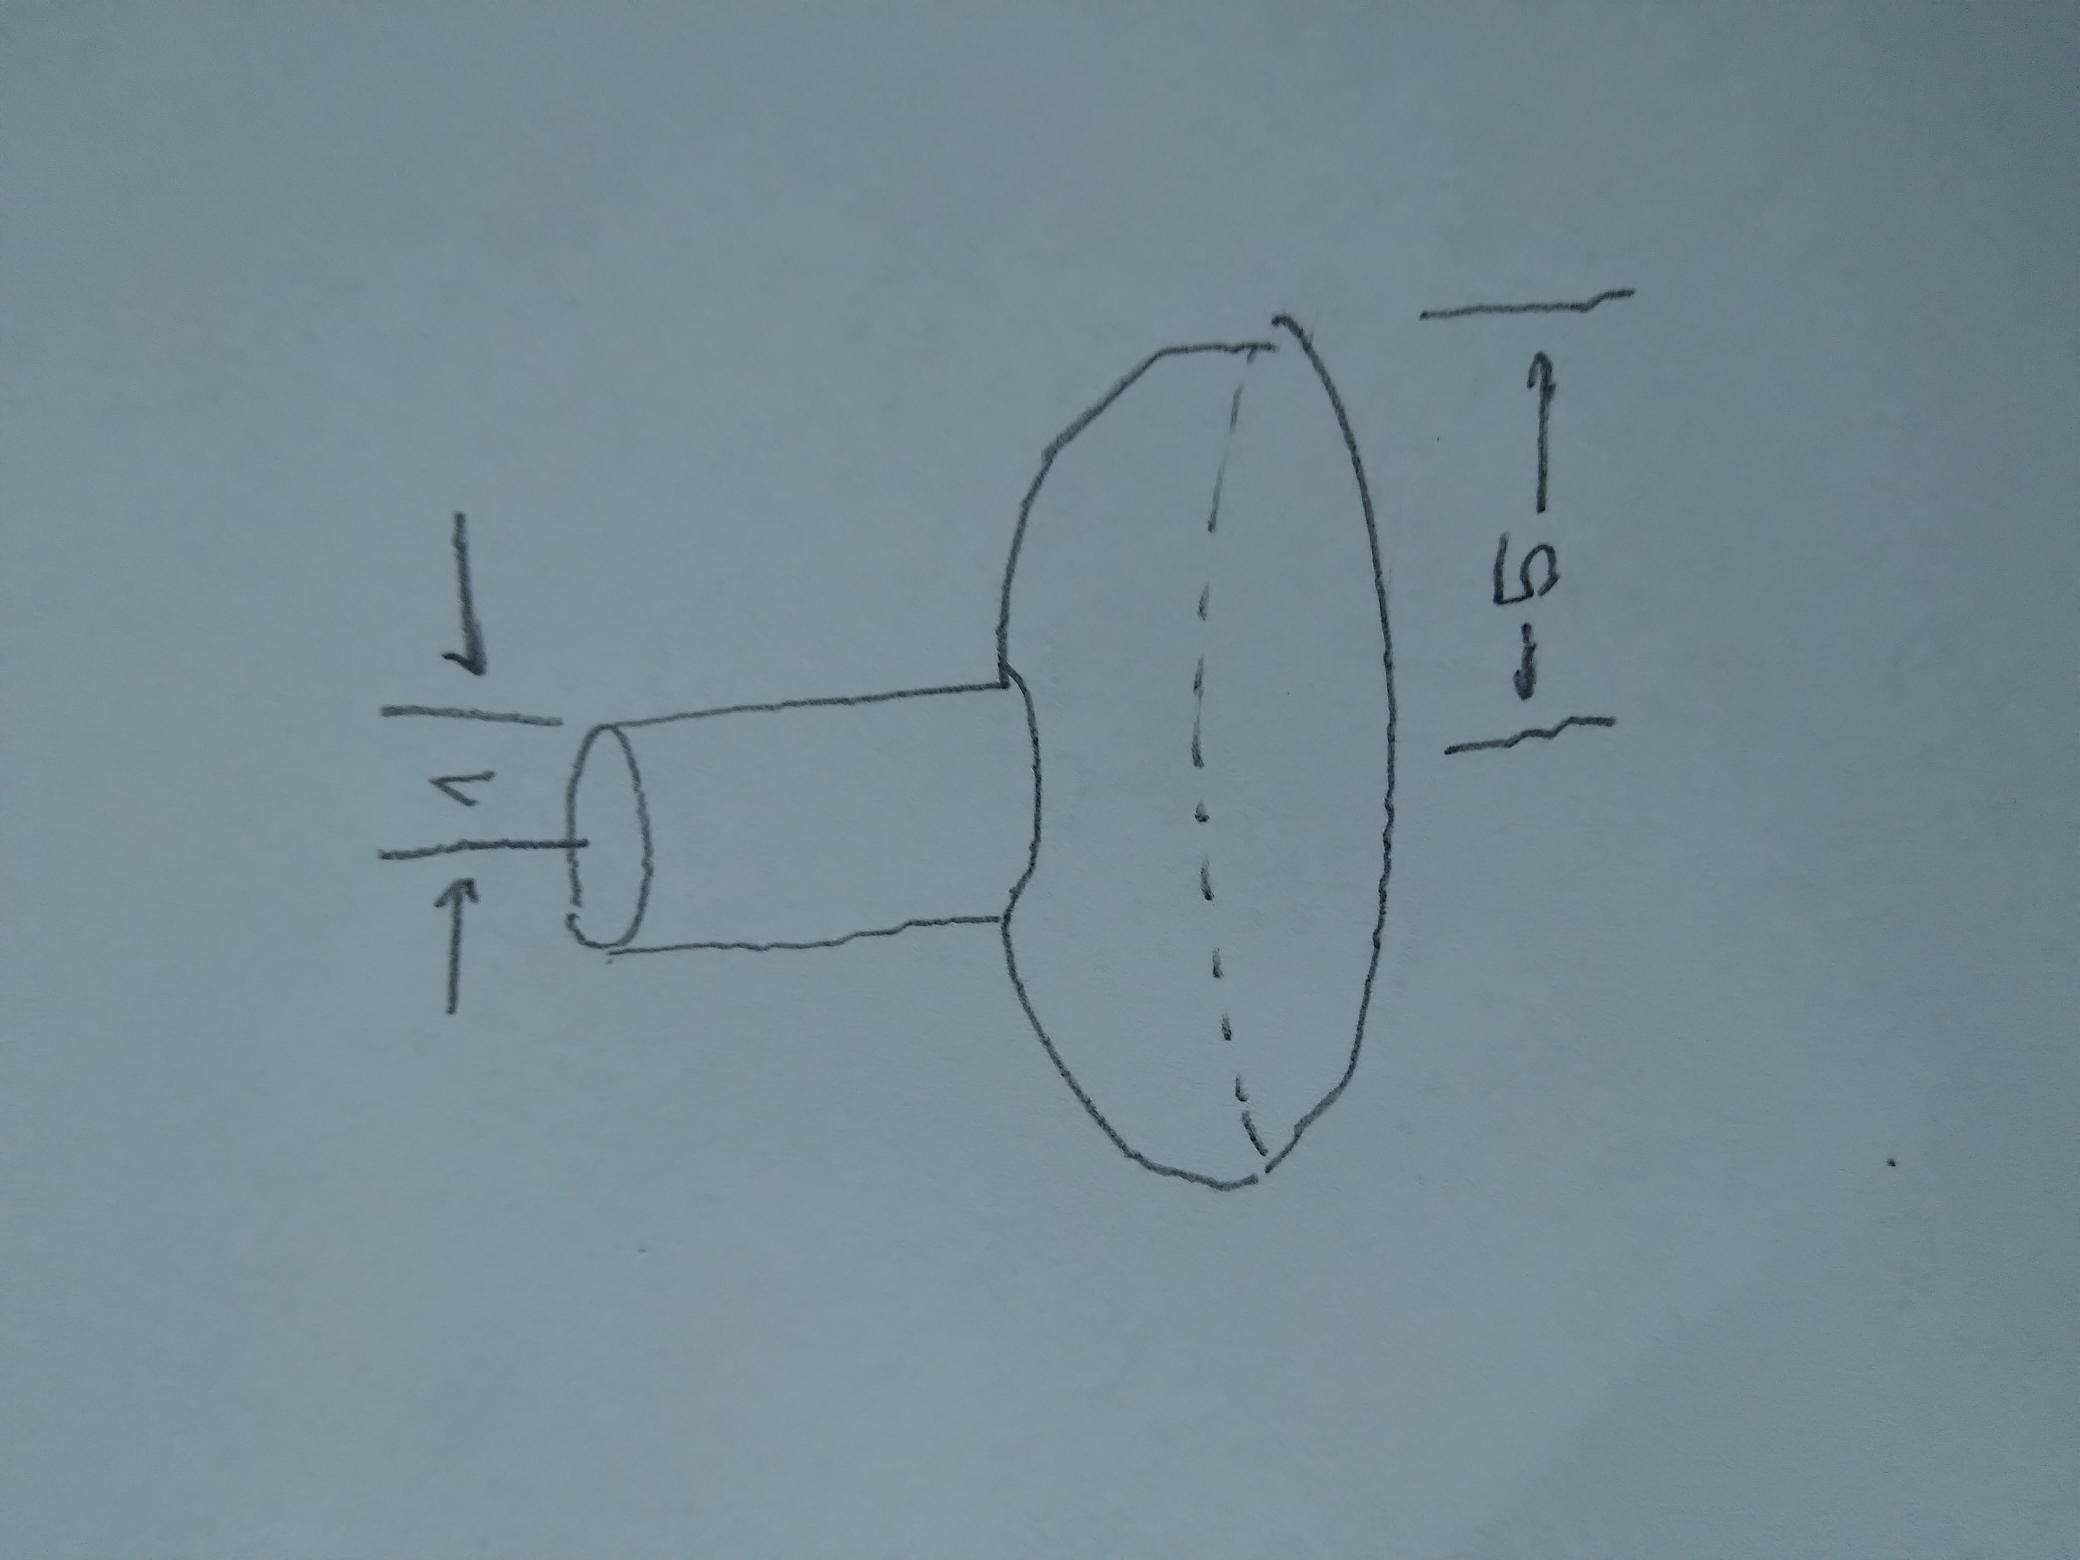
\includegraphics[scale=0.08,angle=-90]{20230824_102843.jpg}
    \end{solution}

    \newpage

    \part[1] Find the numerical value of the volume of the solid generated by revolving 
    the graph of $F$ about the x-axis. You may use strips that
    perpendicular or parallel to the axis of rotation--the choice
    is yours.

    \begin{solution}[2.5in] Let's use strips that are perpendicular to 
        the axis of rotation. We have
        \begin{align*}
          V &= \uppi \int_0^2 (5-x^2)^2 \, \mathrm{dx} + \uppi \int_1^4 \, \mathrm{dx}, \\
            &= \uppi \frac{{{x}^{5}}}{5}- \uppi \frac{10 {{x}^{3}}}{3}+25 x \vert_0^1 +
              x \vert_2^4, \\
            &= \uppi \frac{328}{15} + 3 \uppi, \\
            &= \frac{476 \uppi}{15}.
        \end{align*}
            
       
    \end{solution}

\end{parts}

\newpage
\question Define a function $G$ by 
$G(x) = \begin{cases} 2-x & 0 \leq x \leq 1 \\
                       1  & 1 < x \leq 2
\end{cases}.
$

\begin{parts}

    \part [1] Sketch a graph of $G$. Notice $\dom(G) = [0,2]$,
    so don't extend the graph to the left of zero or to the 
    right of two.

    \begin{solution}[1.5in]
        \begin{center}        
            \includegraphics*[scale=0.3]{desmos-graph(53).png}
        \end{center}
    \end{solution}

    \part [1] The graph of $G$ is revolved about the y-axis, forming
    a solid of revolution. As best you can, draw a picture of 
    this solid.

  It looks like a cylindrical cake with a Hershey kiss on the top.

    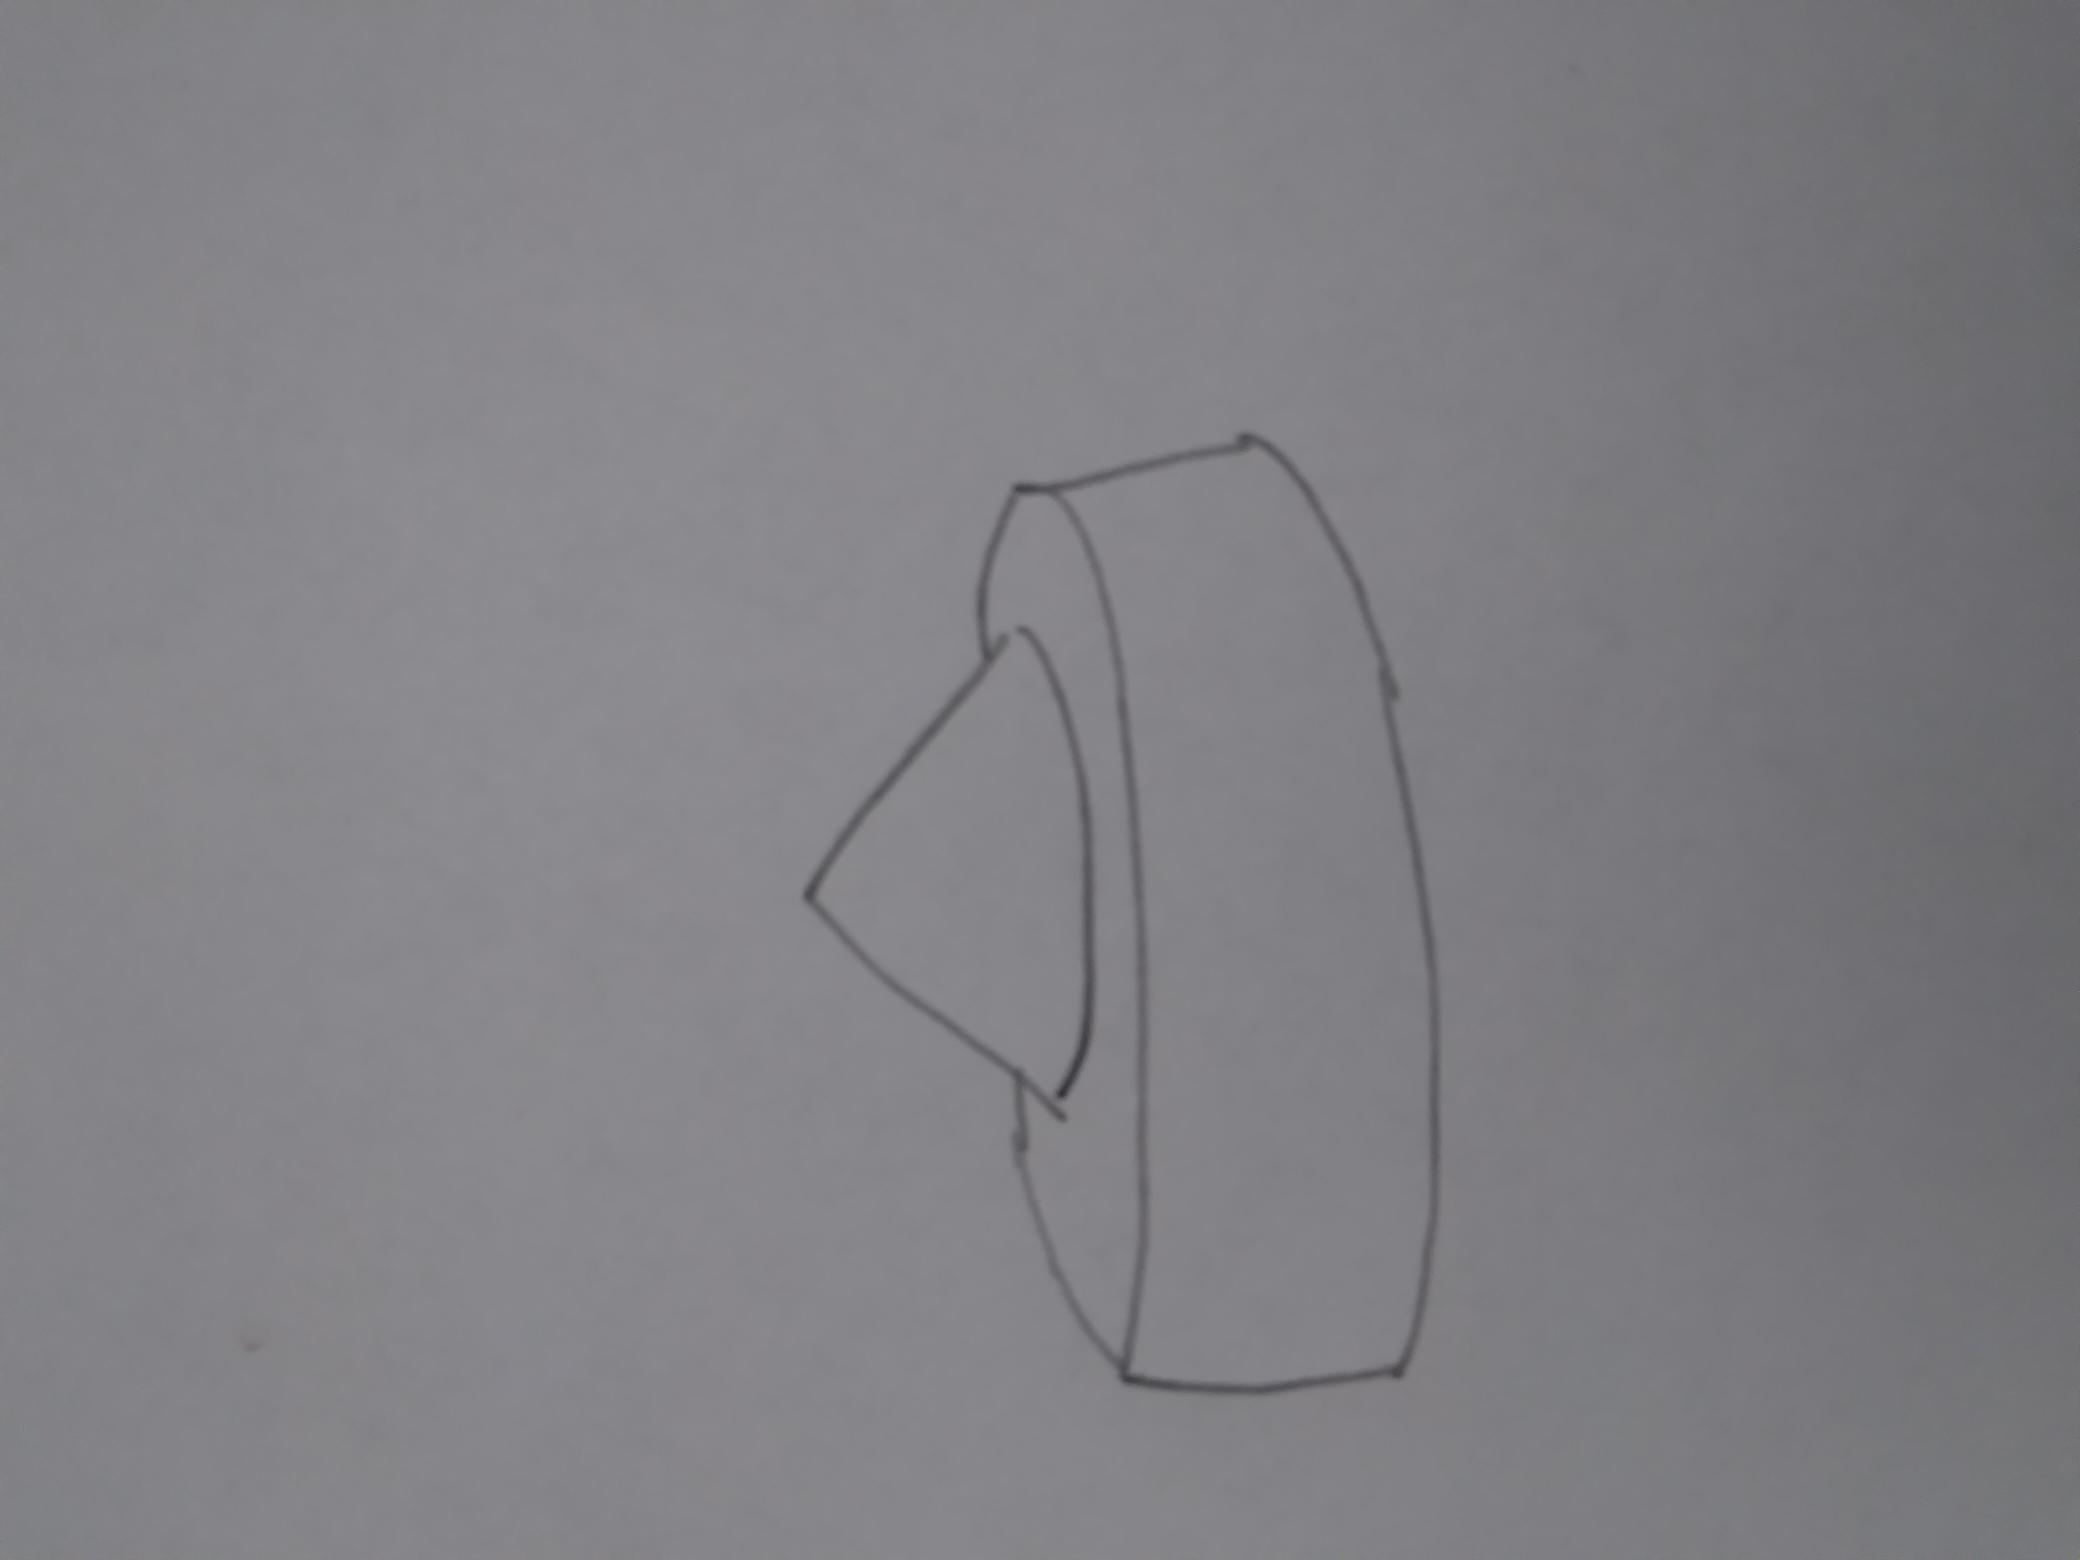
\includegraphics[scale=0.08,angle=-90]{20230824_103250.jpg}
    \newpage
    
    \part [1] Find the numerical value of the volume of the solid generated by revolving 
    the graph of $G$ about the y-axis. You may use strips that
    perpendicular or parallel to the axis of rotation--the choice
    is yours.

    
        \begin{solution}[1.5in] Let's use strips that are parallel to
            the axis of rotation. We have
            \begin{align*}
                V &= 2 \uppi \int_0^1 x (2-x) \, \mathrm{d} x +
                     2 \uppi \int_1^2 x  \, \mathrm{d} x \\
                &= \frac{13 \ensuremath{\uppi} }{3}.
            \end{align*}
    
            
        \end{solution}
  
\end{parts}
\end{questions}

\end{document}

